\documentclass[letterpaper,10pt,twoside]{article}
\usepackage[utf8]{inputenc}

\usepackage{pgfplots}
\usepackage{pgfplotstable}
\pgfplotsset{compat=1.9}
\pgfplotsset{every axis legend/.append style={
    at={(1,1.05)},
                anchor=south east,
                column sep=1ex}}
    
\usepackage{minted}
\usepackage[hidelinks]{hyperref}
\usepackage{caption}
\usepackage{subcaption}


% Title Page
\title{CS 520: Programming Assignment \#1}
\author{Zachary Seymour}


\begin{document}
\maketitle
\section{Problem 1}

\pgfplotstableread{file1.csv}{\chartfile}

\begin{figure}
 \centering
 \begin{tikzpicture}[scale=0.9]
 \begin{axis}[minor tick num=1, xlabel=Issue Queue Size,ylabel=Instructions per Cycle]
  \addplot[black] table [x={IQ},y={bzip2.arg}] {\chartfile};
  \addplot[red] table [x={IQ},y={equake.arg}] {\chartfile};
  \addplot[green] table [x={IQ},y={gcc.arg}] {\chartfile};
  \addplot[blue] table [x={IQ},y={gzip.arg}] {\chartfile};
  \addplot[orange] table [x={IQ},y={mcf.arg}] {\chartfile};
  \addplot[purple] table [x={IQ},y={swim.arg}] {\chartfile};
  \legend{bzip2,equake,gcc,gzip,mcf,swim}
 \end{axis}
\end{tikzpicture}
\caption{Issue Queue Length vs. IPC for various benchmarks}
\label{fig:iqlength}
\end{figure}

As can be seen in \autoref{fig:iqlength}, for each of the benchmarks, the performance (measured by instructions per cycle) increases as we increase the length of the issue queue.  
After it exceeds between sixteen and twenty entries in length, though, the performance increases essentially level out.
Because of instruction latency and dependencies, there will reach a point where only a finite number of instructions will be available to execute in each cycle.
For the given benchmarks, it is likely this point has been reached where we seem the performance gains drop off.
Therefore, no matter how many instructions we allowed to enter the issue queue, we have maxed out the amount that can become ready to execute per cycle.



\section{Problem 2}
\pgfplotstableread[col sep=comma]{2a-ipc.csv}{\firstsub}
\pgfplotstableread[col sep=comma]{2a-hitrate.csv}{\secondsub}
\pgfplotstableread[col sep=comma]{2b-ipc.csv}{\thirdsub}
\pgfplotstableread[col sep=comma]{2b-hitrate.csv}{\fourthsub}
\pgfplotstableread[col sep=comma]{2c-ipc.csv}{\fifthsub}
\pgfplotstableread[col sep=comma]{2c-hitrate.csv}{\sixthsub}
\begin{figure}
 \centering
 \begin{subfigure}[b]{0.45\textwidth}
 \begin{tikzpicture}
   \begin{axis}[minor tick num=1, xlabel=Cache Size,ylabel=Instructions per Cycle,width=\columnwidth]
  \addplot[black] table [x={size},y={bzip}] {\firstsub};
  \addplot[red] table [x={size},y={equake}] {\firstsub};
  \addplot[green] table [x={size},y={gcc}] {\firstsub};
  \addplot[blue] table [x={size},y={gzip}] {\firstsub};
  \addplot[orange] table [x={size},y={mcf}] {\firstsub};
  \addplot[purple] table [x={size},y={swim}] {\firstsub};
 \end{axis}
 \end{tikzpicture}
 \caption{Impacts of changing cache size on IPC.}
 \end{subfigure}
 \qquad
 \begin{subfigure}[b]{0.45\textwidth}
 \begin{tikzpicture}
   \begin{axis}[minor tick num=1, xlabel=Cache Size,ylabel=Hit Rate,width=\columnwidth]
  \addplot[black] table [x={size},y={bzip}] {\secondsub};
  \addplot[red] table [x={size},y={equake}] {\secondsub};
  \addplot[green] table [x={size},y={gcc}] {\secondsub};
  \addplot[blue] table [x={size},y={gzip}] {\secondsub};
  \addplot[orange] table [x={size},y={mcf}] {\secondsub};
  \addplot[purple] table [x={size},y={swim}] {\secondsub};
 \end{axis}
 \end{tikzpicture}
 \caption{Impacts of changing cache size on hit rate.}
 \end{subfigure}
 
 \begin{subfigure}[b]{0.45\textwidth}
  \begin{tikzpicture}
   \begin{axis}[minor tick num=1, xlabel=Cache Associativity,ylabel=Instructions per Cycle,width=\columnwidth]
  \addplot[black] table [x={assoc},y={bzip}] {\thirdsub};
  \addplot[red] table [x={assoc},y={equake}] {\thirdsub};
  \addplot[green] table [x={assoc},y={gcc}] {\thirdsub};
  \addplot[blue] table [x={assoc},y={gzip}] {\thirdsub};
  \addplot[orange] table [x={assoc},y={mcf}] {\thirdsub};
  \addplot[purple] table [x={assoc},y={swim}] {\thirdsub};
 \end{axis}
 \end{tikzpicture}
 \caption{Impacts of changing cache associativity on IPC.}
 \end{subfigure}
 \qquad
 \begin{subfigure}[b]{0.45\textwidth}
 \begin{tikzpicture}
   \begin{axis}[minor tick num=1, xlabel=Cache Associativity,ylabel=Hit Rate,width=\columnwidth]
  \addplot[black] table [x={assoc},y={bzip}] {\fourthsub};
  \addplot[red] table [x={assoc},y={equake}] {\fourthsub};
  \addplot[green] table [x={assoc},y={gcc}] {\fourthsub};
  \addplot[blue] table [x={assoc},y={gzip}] {\fourthsub};
  \addplot[orange] table [x={assoc},y={mcf}] {\fourthsub};
  \addplot[purple] table [x={assoc},y={swim}] {\fourthsub};
 \end{axis}
 \end{tikzpicture}
 \caption{Impacts of changing cache associativity on hit rate.}
 \end{subfigure}
 
  \begin{subfigure}[b]{0.45\textwidth}
  \begin{tikzpicture}
   \begin{axis}[minor tick num=1, xlabel=Cache Line Size,ylabel=Instructions per Cycle,width=\columnwidth]
  \addplot[black] table [x={line},y={bzip}] {\fifthsub};
  \addplot[red] table [x={line},y={equake}] {\fifthsub};
  \addplot[green] table [x={line},y={gcc}] {\fifthsub};
  \addplot[blue] table [x={line},y={gzip}] {\fifthsub};
  \addplot[orange] table [x={line},y={mcf}] {\fifthsub};
  \addplot[purple] table [x={line},y={swim}] {\fifthsub};
 \end{axis}
 \end{tikzpicture}
 \caption{Impacts of changing cache line size on IPC.}
 \end{subfigure}
 \qquad
 \begin{subfigure}[b]{0.45\textwidth}
 \begin{tikzpicture}
   \begin{axis}[minor tick num=1, xlabel=Cache Line Size,ylabel=Hit Rate,width=\columnwidth]
  \addplot[black] table [x={line},y={bzip}] {\sixthsub};
  \addplot[red] table [x={line},y={equake}] {\sixthsub};
  \addplot[green] table [x={line},y={gcc}] {\sixthsub};
  \addplot[blue] table [x={line},y={gzip}] {\sixthsub};
  \addplot[orange] table [x={line},y={mcf}] {\sixthsub};
  \addplot[purple] table [x={line},y={swim}] {\sixthsub};
 \end{axis}
 \end{tikzpicture}
 \caption{Impacts of changing cache line size on hit rate.}
 \end{subfigure}
\caption{Performance impacts of various changes to the cache. (Legend as in \autoref{fig:iqlength})}
\label{fig:cache}
\end{figure}

In \autoref{fig:cache}, we can see the effects of changing various cache parameters on the performance of the processor and its success on finding data in the cache memory.
When we alter the cache size, there is a hit to IPC when the cache is very small, under 8K or so.
We also see the hit rate jump dramatically for most of the benchmarks past this point, from under 80\% to 95\% or more.
Taking these two facts together it would seem the IPC performance takes a hit from the latency of directly accessing memory rather than getting data from the cache, since small cache size means high turnover.

Altering cache associativity does not have as dramatic an effect on either performance or cache hit rates.
Increasing associativity likely benefits throughput at first because it is lowering cache miss latency, as in the first part.
However, the gains are likely offset by the latency caused by searching all possibly locations the data could have been stored due to associativity.
As expected, we seem tapering but constant gains in hit rate from increasing the associativity, as there are more places in the cache to potentially store a given piece of data.

Finally, changing the cache line size, while seemingly have little effect on performance caused great gains in hit rate.
With fixed cache size, increasing the cache line size decreases the number of blocks that can be stored in the cache.
However, it does increase the amount of data stored and each block, as well as the amount of extra data stored in the cache that may be needed in the near future.
Consequently, we get much higher hit rates with long cache lines, since, when we have a miss, the cache also brings in more data around the missed data, which is also likely to be used soon.

\section{Problem 3}
\begin{table}
\pgfplotstabletypeset[
    string type,
    columns/Benchmark/.style={column name=Benchmark, column type={|l}},
    columns/oldest/.style={column name=Oldest-first, column type={|c}},
    columns/position/.style={column name=Position-based, column type={|c}},
    columns/longer/.style={column name=Longer-latency, column type={|c}},
    columns/loads/.style={column name=Loads-first, column type={|c|}},
    every head row/.style={before row=\hline,after row=\hline},
    every last row/.style={before row=\hline\hline, after row=\hline},
    ]{file2.csv}
    \caption{Results of different priority algorithms for ready queue (shown in instructions per cycle).}
    \label{tab:ready}
\end{table}

The data in \autoref{tab:ready} shows the performance results of implementing the various priority algorithms.
The first column shows the data from the oldest-first method, which is the one implemented by default and, thus, our baseline for comparison.
On average, every other algorithm performed worse in terms of instructions per cycle, although the difference between oldest-first and loads-first is negligible.
This is most likely because, when a \texttt{LOAD} was not preselected to be enqueued, the algorithm proceeded as normal.
The longer-latency algorithm performed the worst out of the four.
By giving priority to instructions with long latency, we likely clogged up the pipeline waiting for lengthy instructions to execute.
Similarly, the position-based algorithm probably underperformed because it did not take into account how long an item had been in the issue queue.
For older items, there is a high likelihood another instruction is awaiting their completion, so better performance can be obtained by executing these earlier.



\section{Problem 4}
\begin{figure}
\centering
 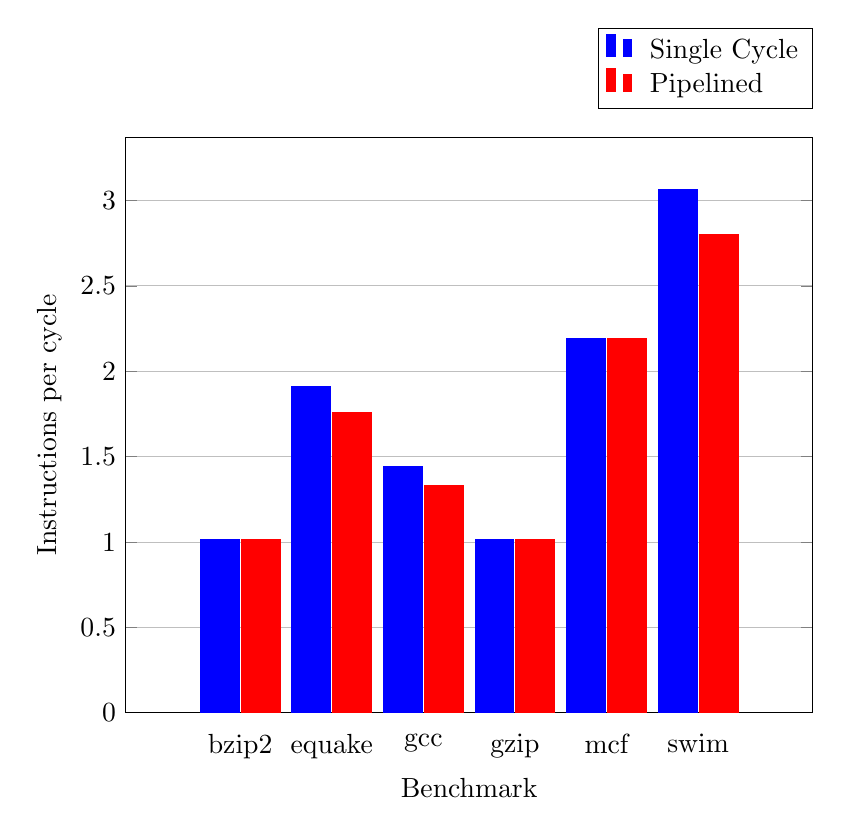
\begin{tikzpicture}
    \begin{axis}[
        width=0.85*\textwidth,
        major x tick style = transparent,
        ybar=2*\pgflinewidth,
        bar width=14pt,
        ymajorgrids = true,
        ylabel = {Instructions per cycle},
        xlabel = {Benchmark},
        symbolic x coords={bzip2,equake,gcc,gzip,mcf,swim},
        xtick = data,
        scaled y ticks = false,
        enlarge x limits=0.25,
        ymin=0,
        legend cell align=left,
        legend style={
                at={(1,1.05)},
                anchor=south east,
                column sep=1ex
        }
    ]
        \addplot[style={blue,fill=blue,mark=none}]
            coordinates {(bzip2,1.0144) (equake,1.9093) (gcc,1.4402) (gzip,1.0144) (mcf,2.1908) (swim,3.0624)};

        \addplot[style={red,fill=red,mark=none}]
             coordinates {(bzip2,1.0144) (equake,1.7579) (gcc,1.3337) (gzip,1.0144) (mcf,2.1907) (swim,2.8017)};
        \legend{Single Cycle, Pipelined}
    \end{axis}
\end{tikzpicture}
\caption{Performance for each benchmark with single-cycle or pipelined wakeup/select stages.}
\label{fig:wakeup}
\end{figure}
The chart shown in \autoref{fig:wakeup} shows the performance impact of pipelining the wakeup/select stages in the processor.
I implemented this in simulation by reversing the calls to \verb|wakeup()| and \verb|selection()| so that \verb|selection| was called first.
This introduced the necessary bubble cycle between the stages.
As can be expected, across most of the benchmarks, this change degraded performance.
With instructions not being selected until a cycle after they are woken, the throughput of the processor drops across all benchmarks.
The bzip2, gzip, and mcf benchmarks all just rely on integer arithmetic, so this is likely why there were no noticeable hits to their performance.

\appendix
\section{Code Listings for Problem 2}
\subsection{Oldest-first}
\begin{minted}[linenos]{c}
static void
readyq_enqueue(struct ROB_entry *rs)	/* RS to enqueue */
{
  struct RS_link *prev, *node, *new_node;

  /* node is now queued */
  if (rs->queued)
    panic("node is already queued");
  rs->queued = TRUE;


  assert(all_operands_spec_ready(rs));


  /* get a free ready list node */
  RSLINK_NEW(new_node, rs);
  new_node->x.seq = rs->seq;

  /* otherwise insert in program order (earliest seq first) */
  /* OLDEST FIRST ISSUE */
  for (prev=NULL, node=ready_queue;
     node && node->x.seq < rs->seq;
     prev=node, node=node->next);

  if (prev)
    {
      /* insert middle or end */
      new_node->next = prev->next;
      prev->next = new_node;
    }
  else
    {
      /* insert at beginning */
      new_node->next = ready_queue;
      ready_queue = new_node;
    }
}
\end{minted}

\subsection{Position-based}
 \begin{minted}[linenos]{c}
static void
readyq_enqueue(struct ROB_entry *rs)	/* RS to enqueue */
{
  struct RS_link *prev, *node, *new_node;

  /* node is now queued */
  if (rs->queued)
    panic("node is already queued");
  rs->queued = TRUE;


  assert(all_operands_spec_ready(rs));


  /* get a free ready list node */
  RSLINK_NEW(new_node, rs);
  new_node->x.seq = rs->seq;

  /* otherwise insert in program order (earliest seq first) */
  /* OLDEST FIRST ISSUE */
  for (prev=NULL, node=ready_queue;
     node && node->x.seq < rs->iq_entry_num;
     prev=node, node=node->next);

  if (prev)
    {
      /* insert middle or end */
      new_node->next = prev->next;
      prev->next = new_node;
    }
  else
    {
      /* insert at beginning */
      new_node->next = ready_queue;
      ready_queue = new_node;
    }
}
 \end{minted}

\subsection{Longer-latency first}
 \begin{minted}[linenos]{c}
static void
readyq_enqueue(struct ROB_entry *rs)	/* RS to enqueue */
{
  struct RS_link *prev, *node, *new_node;

  /* node is now queued */
  if (rs->queued)
    panic("node is already queued");
  rs->queued = TRUE;


  assert(all_operands_spec_ready(rs));


  /* get a free ready list node */
  RSLINK_NEW(new_node, rs);
  new_node->x.seq = rs->seq;
  

  /* otherwise insert in program order (earliest seq first) */
  /* OLDEST FIRST ISSUE */
  for (prev=NULL, node=ready_queue;
     node && node->rs->exec_lat > rs->exec_lat;
     prev=node, node=node->next);

  if (prev)
    {
      /* insert middle or end */
      new_node->next = prev->next;
      prev->next = new_node;
    }
  else
    {
      /* insert at beginning */
      new_node->next = ready_queue;
      ready_queue = new_node;
    }
}  
 \end{minted}

\subsection{\texttt{LOAD} first}
 \begin{minted}[linenos]{c}
  static void
readyq_enqueue(struct ROB_entry *rs)		/* RS to enqueue */
{
  struct RS_link *prev, *node, *new_node;

  /* node is now queued */
  if (rs->queued)
    panic("node is already queued");
  rs->queued = TRUE;


  assert(all_operands_spec_ready(rs));


  /* get a free ready list node */
  RSLINK_NEW(new_node, rs);
  new_node->x.seq = rs->seq;
  
  if (/* load? */
	  ((rs->op) & (F_MEM|F_LOAD)) == (F_MEM|F_LOAD))
  {
    /* insert at beginning */
      new_node->next = ready_queue;
      ready_queue = new_node;
  }
  /* otherwise insert in program order (earliest seq first) */
  /* OLDEST FIRST ISSUE */
  else
  {
  for (prev=NULL, node=ready_queue;
     node && node->x.seq < rs->seq;
     prev=node, node=node->next);

  if (prev)
    {
      /* insert middle or end */
      new_node->next = prev->next;
      prev->next = new_node;
    }
  else
    {
      /* insert at beginning */
      new_node->next = ready_queue;
      ready_queue = new_node;
    }
  }
}
 \end{minted}


\end{document}          
